% !TEX TS-program = XeLaTeX
% use the following command: 
% all document files must be coded in UTF-8
\documentclass{textolivre}
% for anonymous submission
%\documentclass[anonymous]{textolivre}
% to create HTML use 
%\documentclass{textolivre-html}
% HTML compile using make4ht
% $ make4ht -c textolivre-html.cfg -u -x article "fn-in,svg,pic-align"   
%
% See more information on the repository: https://github.com/leolca/textolivre

% Metadata
\begin{filecontents*}[overwrite]{article.xmpdata}
    \Title{El aprendizaje de las tecnologías en el área de lengua castellana y literatura: el proyecto educativo Superpixépolis}
    \Author{Elisabeth Melguizo Moreno}
    \Language{es}
    \Keywords{Aprendizaje \sep Tecnologías emergentes \sep Contenidos digitales \sep Libro de texto \sep Educación primaria \sep Proyecto educativo}
    \Journaltitle{Texto Livre}
    \Journalnumber{1983-3652}
    \Volume{14}
    \Issue{1}
    \Firstpage{1}
    \Lastpage{16}
    \Doi{10.35699/1983-3652.2021.26394}

    \setRGBcolorprofile{sRGB_IEC61966-2-1_black_scaled.icc}
            {sRGB_IEC61966-2-1_black_scaled}
            {sRGB IEC61966 v2.1 with black scaling}
            {http://www.color.org}
\end{filecontents*}

\journalname{Texto Livre: Linguagem e Tecnologia}
\thevolume{14}
\thenumber{1}
\theyear{2021}
\receiveddate{\DTMdisplaydate{2020}{11}{23}{-1}} % YYYY MM DD
\accepteddate{\DTMdisplaydate{2020}{12}{21}{-1}}
\publisheddate{\today}
% Corresponding author
\corrauthor{Elisabeth Melguizo Moreno}
% DOI
\articledoi{10.35699/1983-3652.2021.26394}
% list of available sesscions in the journal: articles, dossier, reports, essays, reviews, interviews, editorial
\articlesessionname{Educação e Tecnologia}
% Abbreviated author list for the running footer
\runningauthor{Melguizo Moreno}
\editorname{Daniervelin Pereira}

\title{El aprendizaje de las tecnologías en el área de lengua castellana y literatura: el proyecto educativo Superpixépolis}
\othertitle{A aprendizagem da tecnologia na área de língua espanhola e suas literaturas: o projeto educativo Superpixépolis}
\othertitle{The learning of technologies in the area of spanish language and literature: the Superpixépolis educational project}

% if there is a third language title, add here:
%\othertitle{Artikelvorlage zur Einreichung beim Texto Livre Journal}

\author[1]{Elisabeth Melguizo Moreno \orcid{0000-0001-6964-964X} \thanks{Email: \url{ely@ugr.es}}}

\affil[1]{Universidad de Granada, Granada, España.}


\addbibresource{article.bib}
% use biber instead of bibtex
% $ biber tl-article-template

% set language of the article
\setdefaultlanguage{spanish}
\setotherlanguage{portuguese}
\setotherlanguage{english}

% for spanish, use:
%\setdefaultlanguage{spanish}
\gappto\captionsspanish{\renewcommand{\tablename}{Tabla}} % use 'Tabla' instead of 'Cuadro'
\AfterEndPreamble{\crefname{table}{tabla}{tablas}\Crefname{table}{Tabla}{Tablas}}

% for languages that use special fonts, you must provide the typeface that will be used
% \setotherlanguage{arabic}
% \newfontfamily\arabicfont[Script=Arabic]{Amiri}
% \newfontfamily\arabicfontsf[Script=Arabic]{Amiri}
% \newfontfamily\arabicfonttt[Script=Arabic]{Amiri}
%
% in the article, to add arabic text use: \textlang{arabic}{ ... }

\usepackage{multirow}
\begin{document}
\maketitle

\begin{polyabstract}
\begin{abstract}
Las tecnologías de la información y la comunicación han formado parte de los currículos de enseñanza ante la demanda de una nueva sociedad digital. En esta contribución se estudia el aprendizaje de las tecnologías en el área de Lengua Castellana y Literatura durante la Educación Primaria, en el proyecto educativo Superpixépolis de la editorial Edelvives. Se desarrolla un enfoque metodológico mixto; cualitativo, que gira en torno al análisis de los contenidos digitales en 16 libros de texto, por parte de docentes expertos en la materia; y cuantitativo, mediante el programa IBM SPSS Statistics 26.0, a través de un análisis descriptivo de las siguientes variables: curso, tipo de contenido digital, bloque del libro, complejidad de la actividad, destrezas lingüísticas y agrupamientos. Los resultados han mostrado una presencia importante de actividades digitales en los libros de texto (N= 89) correspondientes, en su mayoría, a segundo y tercer ciclo de Primaria; trataban de búsquedas de información en Internet o consulta de fuentes digitales; pertenecían al bloque de Técnicas de estudio (Repasa o Literatura); eran de un nivel intermedio; trabajaban las destrezas escritas y se planteaban de forma individual. Se concluye que el aprendizaje de contenidos tecnológicos en los libros de texto aún debe mejorar, puesto que no fomenta apenas las destrezas orales ni el aprendizaje colaborativo y tampoco posee identidad propia, ya que se desarrolla fundamentalmente en técnicas de estudio, repaso o literatura.

\keywords{Aprendizaje \sep Tecnologías emergentes \sep Contenidos digitales \sep Libro de texto \sep Educación primaria \sep Proyecto educativo}
\end{abstract}

\begin{portuguese}
\begin{abstract}
As Tecnologias da Informação e Comunicação (TICs) tem feito parte dos currículos diante das necessidades de uma nova sociedade digital. Nesse sentido, se estuda a aprendizagem de tecnologia na área de língua espanhola e suas literaturas durante o ensino fundamental no projeto educativo Superpixépolis da editora Edelvives. Com uma metodologia mista: qualitativa, que gira em torno da análise de conteúdos digitais de 16 livros didáticos por parte do professor de cada disciplina; e quantitativo usando o programa IBM SPSS Stadistics 26.0, através de uma análise descritiva das seguintes variáveis: curso, tipo de conteúdo digital, sessão do livro, complexidade da atividade, habilidade linguística e agrupamentos. Os resultados mostraram uma presença importante de atividades digitais no livro didático (N=89), a maioria no quinto e sexto ano do ensino fundamental, tratava-se da busca de informações na internet ou consulta de fontes digitais, pertenciam ao bloco de técnicas de estudo (Revisão ou Literatura), eram de um nível intermediário, trabalhavam as habilidades escritas de forma individual. Conclui-se a aprendizagem de conteúdo tecnológico nos livros didáticos ainda precisa melhorar, tendo em vista que não desenvolve as habilidades orais nem a aprendizagem colaborativa e tampouco possui identidade própria, já que se desenvolve fundamentalmente em técnicas de estudo, revisão ou literatura.

\keywords{Aprendizagem \sep Tecnologias emergentes \sep Conteúdos digitais \sep Livro didático \sep Ensino fundamental \sep Projeto educativo}
\end{abstract}
\end{portuguese}

\begin{english}
\begin{abstract}
Education and Information technologies have been part of the teaching curricula due to the demands of a new digital society. In this contribution, a study has been carried out regarding the learning of technologies in the area of "Spanish Language and Literature” during Primary Education following the Superpixel educational project by the Edelvives publishing company. A mixed methodological approach was developed: firstly, qualitative, linked to the analysis of digital contents of 16 textbooks, by expert teachers in the matter; and, secondly, quantitative, through the IBM SPSS Statistics 26.0 program, following a descriptive analysis of the following variables: course, type of digital content, book section, complexity of the activity, linguistic skills and groupings. The results have shown an important presence of digital activities in textbooks (N= 89) corresponding, mostly, to the second and third cycles of Primary Education. These activities involved searching for information online; were part of the Study Skills section (Revision or Literature); were of an intermediate level; focused on writing skills, and were designed for individual work. It is concluded that learning of technological contents from textbooks is yet to be improved since it barely focuses on neither oral skills nor collaborative learning apart from not having its own identity since it is developed mostly through study techniques, revisions, and literature.

\keywords{Learning \sep Emerging technologies \sep Digital contents \sep Textbook \sep Primary education \sep Educational project}
\end{abstract}
\end{english}

% if there is another abstract, insert it here using the same scheme
\end{polyabstract}


\section{Introducción y estado de la cuestión}\label{sec-intro}
Es una realidad que las tecnologías de la información y la comunicación (TIC) han invadido nuestro día a día. Los centros educativos se encuentran en la tesitura de cómo trabajar contenidos digitales en el aula, razón por la cual deben forman parte del currículo del sistema educativo como saberes susceptibles de ser enseñados. En el Real Decreto 126/2014, de 28 de febrero, por el que se establece el currículo básico de la Educación Primaria, se establece, entre los objetivos a adquirir en la etapa el de: “i) iniciarse en la utilización, para el aprendizaje, de las Tecnologías de la Información y la Comunicación desarrollando un espíritu crítico ante los mensajes que reciben y elaboran” \cite[p. 19354]{ministerio_de_educacion_y_ciencia_real_2014}. Igualmente, es interesante que, en la determinación de los elementos transversales de Educación Primaria, se insista en que “1. Sin perjuicio de su tratamiento específico en algunas de las asignaturas de cada etapa […] las Tecnologías de la Información y la Comunicación, el emprendimiento y la educación cívica y constitucional se trabajarán en todas las asignaturas” \cite[p. 19356]{ministerio_de_educacion_y_ciencia_real_2014}. En concreto, en el área de Lengua Castellana y Literatura (LCyL), dicho decreto afirma que, pese a que la finalidad de esta área en Educación Primaria es el desarrollo de las cuatro destrezas básicas de uso de la lengua (escuchar, hablar, leer y escribir), su adquisición debe realizarse aunando la lectura, comprensión y reflexión de diferentes tipos de textos, pero considerando la “realidad cambiante de un individuo que vive inmerso en una sociedad digital y que es capaz de buscar información de manera inmediata a través de las Tecnologías de la Información y la Comunicación” \cite[p. 19378]{ministerio_de_educacion_y_ciencia_real_2014}.

Los bloques de contenido del área de Lengua Castellana y Literatura determinan, por tanto, el desarrollo de las TIC de formas diversas en el Real Decreto 126/2014. En el Bloque 1 (Comunicación oral: escuchar y hablar) se propone la integración de las tecnologías en el aula, de modo que favorezcan un planteamiento integral de estrategias que van desde el análisis de discursos y debates audiovisuales hasta la evaluación de discursos propios y ajenos grabados y proyectados \cite[p. 19379]{ministerio_de_educacion_y_ciencia_real_2014}. Por otro lado, en la Orden de 17 de marzo de 2015, por la que se desarrolla el currículo correspondiente a la Educación Primaria en Andalucía, se alude en las orientaciones metodológicas al uso de las TIC como instrumento facilitador para desarrollar el plan de estudios. Por esta razón, el objetivo seis del área de LCyL de la Orden de 17 de marzo de 2015 es: “aprender a utilizar todos los medios a su alcance, incluida las nuevas tecnologías, para obtener e interpretar la información oral y escrita, ajustándola a distintas situaciones de aprendizaje” \cite[p. 157]{junta_de_andalucia_orden_2015}. 

Las tecnologías de la información y la comunicación están inmersas en nuestra vida cotidiana y, por ende, deben formar parte del contexto educativo ante las demandas sociales \cite{gutierrez_fresned_mejora_2016}. Han sido diferentes los organismos internacionales, como la UNESCO \cite{unesco2010} y europeos, como la \textcite{comisioneuropea2013}, los que han recomendado en sus informes la inclusión de las tecnologías en educación, a través de estándares sobre el desarrollo de la competencia digital. Las TIC, por tanto, abren un nuevo panorama educativo, así como un amplio abanico de posibilidades para la mejora de los procesos de enseñanza-aprendizaje. De hecho, una de las competencias fundamentales que deben adquirir los alumnos es la digital, ya que ofrece múltiples ventajas de formación y aprendizaje personal. \textcite{gairin_sallan_cambio_2009} manifiesta que, entre las características de nuestra sociedad contemporánea, destaca el continuo cambio que experimenta y el protagonismo que tienen las tecnologías de la información y la comunicación. De manera que una sociedad en cambio permanente exige de procesos y organizaciones adaptables, que revisen sus formas de actuar de acuerdo con las cambiantes necesidades del entorno.

Los niños, desde edad temprana, viven en lo que \textcite[p. 6]{sara_malo_2010} denominan “infancia de los medios”, puesto que están imbuidos por medios electrónicos y audiovisuales que determinan sus experiencias. Hacen un uso de las TIC que, indirectamente, amplía sus relaciones interpersonales y los dirige hacia nuevas formas de expresión y comunicación \cite{ortega-ruiz_towards_2014}. De ahí que su alfabetización digital sea estrictamente necesaria \cite{berzosa_ramos_tic_2015}. 

En 2006, la Comisión Ministerial para el estudio de la renovación de las metodologías educativas en las universidades españolas indicó que era necesaria una reforma de los métodos para abordar la actualización de la oferta formativa \cite{ministerio_de_educación_ciencia_2006}. Con el panorama del Espacio Europeo de Educación Superior en aquel tiempo, se destacaba el papel de las TIC como motor de cambio \cite{carrasco_pradas_tic_2005}, que permitieran el desarrollo de distintas tareas. No obstante, algunos estudios \cite{carrera_farran_identificacion_2012} muestran que en realidad el profesorado no se siente capacitado o competente, en muchas ocasiones, para trabajar la competencia digital en el aula, aunque valora su potencial para llevar a cabo la referida y necesaria renovación metodológica \cite{prendes_espinosa_competencias_2013}. En este sentido, \textcite[p. 1489]{agreda_montoro_formacion_2016} afirman que "la adquisición de la competencia digital se hace a partir de la experimentación propia y autodidacta"; sin embargo, la participación del profesorado en cursos de formación presenciales obtiene una mayor representación y escala o nula la formación para el uso de los dispositivos inteligentes como recurso didáctico. 

Por otro lado, diferentes autores \cite{diaz_lazaro_redes_2013, dahlstrom__2014} señalan las ventajas del uso de aplicaciones y herramientas de la Web 2.0 en el aprendizaje del alumno y, más si cabe, en la creación de un espacio de colaboración, donde el estudiante aprende, fundamentalmente, de sus compañeros, generándose un clima de aprendizaje activo, autónomo y colaborativo. 

De igual forma, resulta relevante el amplio abanico de posibilidades que ofrece la escritura digital en el ámbito escolar frente a la escritura manual \cite{vera_castro_tics_2012}, además de la motivación para el alumnado de teclear frente a escribir un texto manuscrito. El uso de los procesadores de textos para la realización de tareas es ya algo habitual en determinadas actividades del aula de primaria. Además, diversos estudios han demostrado los grandes beneficios que posee el aprendizaje de la letra cursiva, donde el cerebro establece una especialización por áreas que integra la sensación, el control de movimiento y el razonamiento \cite{james_role_2009, james_effects_2012}. 

Asimismo, la aparición de las TIC en el currículo de Educación Primaria ha suscitado la necesidad de analizar su presencia en manuales. Los estudios sobre el libro de texto y su utilidad en la enseñanza han estado presentes desde tiempo atrás \cite{escudero_munoz_investigacion_1983, valls_montes_manuales_1998, choppin_les_2002, escolano_benito_manual_2009, rodriguez_rodriguez_digital_2015, villalain_benito_proyecto_2000}, con el Proyecto Manes, entre otros). Ahora bien, \textcite{san_martin_alonso_controversias_2018} cuestionan si realmente tiene futuro el libro de texto o si será desplazado por contenidos digitales en distintos formatos, entre ellos algunos ya presentes como vídeos tutoriales de contenidos curriculares en YouTube, piezas elaboradas por profesores, blogs y materiales propios, contenidos escolares en formato de videojuegos o concursos, etc. Han surgido nuevos artefactos que cambian el modo de acceso al texto. Incluso los autores mencionados insisten en que: "el denominado contenido digital propone una relación diferente con los significados, mucho más lúdicos, fragmentados y cambiantes, justo el tipo de relación que fomenta el actual consumo del ocio y el entretenimiento, mucho más icónico que alfabético" \cite[p. 8]{san_martin_alonso_controversias_2018}. Muchos de los estudiantes del trabajo de estos investigadores manifiestan una clara preferencia por los dispositivos digitales frente a los libros de texto tradicionales.

Es importante, pues, analizar de qué forma se ha producido la necesaria reestructuración didáctica en las aulas. Para ello, se ha realizado un estudio pormenorizado de todos los libros de Lengua Castellana y Literatura de la etapa de educación primaria por cursos (1.º a 6.º) y trimestres (1.º, 2.º y 3.º) del proyecto educativo Superpixépolis de Edelvives \cite{araya_olazaran_lengua_2014-1,araya_olazaran_lengua_2014, araya_olazaran_lengua_2015-1,araya_olazaran_lengua_2015-2, araya_olazaran_lengua_2015-3,araya_olazaran_lengua_2015}, con la finalidad de verificar el tipo de contenidos digitales que aparecen en ellos y su mayor o menor presencia en función del bloque del libro al que pertenecen, la complejidad de la actividad, las destrezas que desarrollan y el agrupamiento que requieren.

\section{Metodología}\label{sec-metodologia}
Se ha realizado una investigación de tipo mixto, cualitativa y cuantitativa. En cuanto al estudio cualitativo se ha usado la metodología de análisis de contenido de los libros de texto, considerando esta técnica como “un conjunto de procedimientos estricto y sistemático para el análisis riguroso, el examen y la verificación de los contenidos de datos estrictos” \cite[p. 563]{cohen_research_2011}.

Para realizar este estudio de carácter descriptivo e interpretativo se definieron como unidades de análisis aquellas actividades o explicaciones teóricas que trataban sobre contenidos digitales en los 18 cuadernillos de Lengua Castellana y Literatura de Educación Primaria (tres por cada curso, correspondientes a los tres trimestres) del proyecto Superpixépolis de la editorial Edelvives. Se analizaron minuciosamente y se realizó su categorización mediante una triangulación de expertos en Didáctica de la Lengua Española. Se descartaron las unidades de análisis que no trabajaban las tecnologías, 2, en particular (el primer trimestre de 1.º y 2.º curso). Por tanto, el estudio ha considerado 16 libros de texto, que se referencian al final de este artículo. 

Concretamente, se realizaron dos tipos de análisis: uno con categorías preestablecidas en la literatura y de forma explícita en los libros de texto (curso, bloque del libro, destrezas, complejidad de la actividad y agrupamientos); y otro análisis de categorías emergentes (como el tipo de contenidos digitales), que requería de un estudio en profundidad de los manuales. 

Para analizar los resultados se tuvieron en cuenta las siguientes categorías preestablecidas:  

\begin{itemize}
    \item Curso: es la variable de estratificación de la muestra (desde 1.º a 6.º de educación primaria).
    \item Bloque del libro: en este caso, de detalla el bloque del libro al que pertenecen los contenidos digitales. Concretamente, los bloques de los manuales han sido recodificados en los siguientes: bloque 1. Técnicas de estudio; bloque 2. Comprensión y expresión oral; bloque 3. Repasa; bloque 4. Literatura; bloque 5. Conocimiento de la lengua; bloque 6. Expresión escrita; bloque 7. Comprensión lectora y lectoescritura y bloque 8. Bloques especiales (Emprendo y aprendo, Cooperamos para aprender, Revista SPX y Conquista PISApolis, entre otros). 
    \item Destrezas o habilidades lingüísticas: \textcite{cassany_ensenar_1994} consideran las siguientes destrezas lingüísticas: expresión y comprensión oral y expresión y comprensión escrita, correspondientes a hablar, escuchar, escribir y leer; también presentes en el currículo de Educación Primaria (Real Decreto 126/2014 y Orden de 17 de marzo de 2015) \cite{ministerio_de_educacion_y_ciencia_real_2014, junta_de_andalucia_orden_2015}. Dichas destrezas fueron recodificadas en el análisis en tres grupos: 1. Destrezas escritas; 2. Destrezas orales; 3. Ambas destrezas.
    \item Complejidad de la actividad\footnote{En relación con la complejidad de la actividad, conviene aclarar que los niveles básico, intermedio y avanzado del DigComp 2.1 \cite{carretero_2018} se tienen en cuenta en función de la complejidad de las tareas a desarrollar en cada una de las actividades que se proponen en los distintos cursos; de ahí que no haya una progresión exacta correlativa del nivel A1 al nivel A2 del MCER, a medida que avanzan los cursos.}: para esta clasificación se ha tenido en cuenta el Marco Europeo de Competencias digitales para la ciudadanía (DigComp 2.1) \cite{carretero_2018}. De los 8 niveles de aptitud que considera, solamente nos interesa el área de competencia 1 (Información y alfabetización digital) y, concretamente, el subepígrafe 1.2. “Evaluar datos, información y contenidos digitales”, que pretende “analizar, comparar y evaluar de forma crítica la fiabilidad y seriedad de recursos de datos, información y contenido digital. Analizar, interpretar y evaluar de forma crítica datos, informaciones y contenidos digitales” (párr. 1). Esta evaluación se basa en varios niveles: básico (1), intermedio (2), avanzado (3) y altamente especializado. Dado que el estudio que se presenta se centra en educación primaria, no se ha tenido en cuenta el nivel altamente especializado, sino que solo se han considerado los tres primeros. Igualmente es de recibo mencionar que \textcite{gisbert_da_cruz_niveles_2011} estableció una correspondencia entre los niveles del MCER y los del Sistema educativo español y, para el ámbito educativo que nos ocupa (Educación Primaria), establecía la siguiente correspondencia: 1.º: A1.1; 2.º: A1.2; 3.º: A1.3; 4.º: A1.4; 5.º: A2.1 y 6.º: A2.2. Por tanto, los niveles del DigComp 2.1 considerados se corresponden, como máximo, con un nivel A2.2 del MCER, que en este caso sería lo que antes se ha denominado nivel avanzado.
    \item Agrupamientos: es importante también determinar si los contenidos digitales que aparecían en las actividades requieren que los estudiantes trabajen de forma individual (1), por parejas (2), pequeños grupos (3) o varios tipos de agrupamiento (4).
\end{itemize}

Por otro lado, el análisis de categorías emergentes consideró solamente la variable tipo de contenidos digitales. Se describen los contenidos relacionados con la comunicación digital que se tratan en la explicación teórica o en las actividades de los libros por trimestres y cursos (1.º- 6.º). Dichos contenidos se han agrupado en categorías que emergen del análisis y se muestran en el epígrafe de resultados en forma de bloques temáticos.

Por lo que respecta al estudio cuantitativo, se ha utilizado el software IBM SPSS Statistics 26.0 para realizar un estudio descriptivo de las categorías de respuesta, centrado principalmente en la obtención de frecuencias y tablas de contingencia.  

En cuanto a los instrumentos utilizados para el análisis previo de contenido de los libros de texto de Lengua Castellana y Literatura, se diseñaron unas hojas de registro ad hoc, de elaboración propia, mediante las que se detallaban en profundidad las categorías preestablecidas y la emergente del análisis. A continuación se presenta una de las tablas modelo utilizada (\cref{tbl01}) con varias actividades representativas del proyecto educativo sobre el ciberacoso, el uso de mensajes en teléfonos móviles y pantallas táctiles correspondientes a 4.º y 6.º de Primaria.  

\clearpage
\begin{small}
\begin{longtable}{p{0.222\textwidth}p{0.22\textwidth}p{0.22\textwidth}p{0.22\textwidth}}
\caption{Tabla modelo para el análisis previo de contenido de los libros de texto del proyecto educativo Superpixépolis.}
\label{tbl01}
\\
\toprule
 & \multicolumn{3}{c}{Curso y trimestre} \\
 & 4.º, 3.º & 6.º, 1.º & 6.º, 2.º \\
\midrule
Actividades &
Por grupos buscad información sobre el ciberacoso y traed a clase algún ejemplo concreto que encontréis en Internet y que haya ocurrido últimamente. Después, reflexionad conjuntamente en el grupo y comentad vuestras conclusiones con el resto de la clase. &
Lee estos mensajes de teléfono móvil. Responde a estas preguntas: ¿Quiénes conversan? ¿Sobre qué tema lo hacen? ¿Cuánto dura la conversación? Fíjate en los términos destacados y di a qué clase de palabra acompañan y qué función cumplen: Es la historia de tres astronautas. Di si la palabra destacada en la siguiente oración sustituye a un nombre, y, si es así, a cuál: Carlos y yo vamos al cine esta tarde. &
Realiza un trabajo en grupo sobre las pantallas táctiles. Para ello, investigad en Internet y seguid este guion. ¿De qué están hechas? ¿Cuándo se inventaron? ¿Cómo funcionan? ¿Cuál es su finalidad? ¿Cuáles son los últimos avances? ¿Qué crees que pasará en el futuro? \\
Bloque del libro y título de la sección &
Emprendo y Aprendo. &
Conoce la lengua. \textit{Mensajes de teléfono móvil} (no explícito). &
Técnicas de estudio. \textit{La búsqueda de información en Internet}. Club de lectura. \\
Destrezas &
Comprensión y expresión escrita y expresión y comprensión oral. & 
Comprensión escrita, expresión oral, expresión escrita. &
Comprensión escrita y expresión escrita (no explícito). \\
Complejidad de la actividad & Nivel avanzado & Nivel intermedio & Nivel avanzado \\
Agrupamientos & Grupal. & Individual y por parejas o grupos & Grupal. \\
Tipo de contenidos digitales & 
Búsqueda de información en Internet sobre el ciberacoso. &
Lectura e interpretación de mensajes de teléfono móvil (WhatsApp-no explícito). &
Investigación en Internet sobre pantallas táctiles. \\
\bottomrule
\source{elaboración propia.}
\end{longtable}
\end{small}

%essa tabela ficou desconfigurada. São 4 colunas.

\section{Análisis y resultados}\label{sec-analisis}
Antes de todo, conviene aclarar la estructura que presentan los libros de texto de Lengua Castellana y Literatura del proyecto Superpixépolis considerados en este estudio. Se puede afirmar que los manuales de 1.º y 2.º curso no ofrecen instrucciones sobre cómo se usa el libro, sino que directamente se muestra el índice y la presentación de los personajes del Planeta Pixépolis y del Planeta Tierra; en cambio en el resto sí. Así pues, en el libro de 1.º aparecen los siguientes bloques: Comunicación oral (comprensión y expresión oral), Lectoescritura, Conocimiento de la lengua (vocabulario, gramática y ortografía), Expresión escrita, Escritura y Literatura. En 2.º se suprime el bloque de Lectoescritura y Escritura; el resto son idénticos. En 3.º, 4.º, 5.º y 6.º se introducen los bloques de Técnicas de estudio y de Literatura; el resto, permanecen igual. Además, hay bloques específicos que se incluyen cada cuatro unidades: Cooperamos para aprender, Conquista PISApolis, Proyecto PBL, Emprendo y Aprendo, Club de lectura o Anexos complementarios.

Seguidamente, se exponen los resultados más significativos que ha revelado esta investigación.  

En primer lugar, se ha advertido que los contenidos digitales que aparecen en los libros de texto analizados se pueden agrupar en los siguientes bloques temáticos (\cref{Fig01}):  

\begin{figure}[htbp]
 \centering
 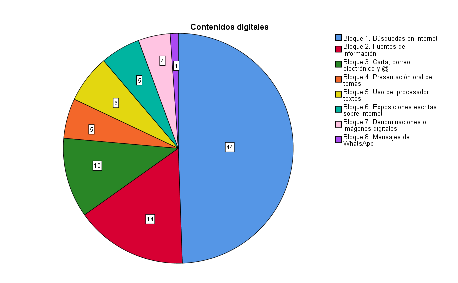
\includegraphics[width=0.85\textwidth]{Fig01.eps}
 \caption{Bloques temáticos de los contenidos digitales.}
 \label{Fig01}
 \source{elaboración propia.}
\end{figure}

Como se puede observar en el \cref{Fig01}, hay 44 actividades que se corresponden con el Bloque temático 1. Consultas o búsquedas de información en Internet (para extraer datos, interpretar información, relacionar investigaciones concretas, hacer lecturas de formularios, blogs, páginas web; realización de traducciones o audiciones de poemas u otros); seguidamente, encontramos 14 actividades del Bloque temático 2. Fuentes de información digitales (periódicos, revistas, enciclopedias digitales, diccionarios, buscadores, etc.) y 10 pertenecientes al Bloque 3. La carta, el correo electrónico y el símbolo de arroba. Mucha menor presencia tienen los bloques 4, 5, 6 y 7 correspondientes a la presentación informática/digital (oral) de un tema; el uso del procesador de textos. Tablas y gráficos (escritura de cuentos a ordenador, anuncios sobre productos); exposiciones escritas sobre Internet (utilidad de Internet, búsqueda de información en la red, utilidad de móviles, tabletas y ordenadores, ciberdelitos y ciberacosos, uso desaconsejable del móvil en determinados contextos) y denominaciones e imágenes de las tecnologías (“teléfono” o “teclado”), que solamente representan a 5, 6, 5 o 4 actividades, respectivamente, en los libros. Finalmente, se encuentra una sola actividad en el bloque temático 8 dedicada a la lectura e interpretación de mensajes de teléfonos móviles (uso de WhatsApp). 

Tanto por la presencia de los contenidos referidos como por la forma en que se trabajan hay una coincidencia con lo expuesto en el currículo de educación primaria, puesto que se afirma que las TIC deben favorecer:  

\begin{quote}
    La adquisición de destrezas orales y escritas en diferentes aspectos: vocabulario, ortografía correcta, redacción de textos, presentaciones adecuadas; relaciones interpersonales, etc. En este sentido, será conveniente la formación del alumnado con respecto a programas educativos informáticos, programas de gestión (procesadores de texto, gestores de correo) e internet, etc. […], puesto que los recursos que nos ofrecen la tecnología son un medio para la construcción del conocimiento a la par de herramientas motivadoras en la elaboración de tareas y proyectos de creación, investigación, análisis, selección y tratamiento de la información. \cite[p. 153]{junta_de_andalucia_orden_2015}.
\end{quote}

Por otro lado, la evolución en la incorporación de dichos contenidos digitales en los libros de Lengua Castellana y Literatura del proyecto Superpixépolis para educación primaria ha sido progresiva aunque nada equilibrada por cursos, ya que es en 4.º (37.1 \%) y en 6.º (23.6 \%) donde más actividades de contenido digital se presentan (Tabla 2). Por tanto, se podría decir que la mayoría de las tareas tecnológicas de este proyecto aparecen fundamentalmente en el segundo ciclo (49), seguido del tercero (34); puesto que en el primer ciclo, solo se evidencian 6 actividades digitales.

\begin{table}
\caption{Actividades por curso.}
\label{tbl02}
\small
\centering
\begin{tabular}{clcc}
\toprule
 & & \textbf{Frecuencia} & \textbf{Porcentaje} \\
\midrule
\multirow{7}{*}{\textbf{Cursos}} & {1.º} & 3 & 3.4 \\
 & 2.º            & 3           & 3.4  \\ 
 & 3.º            & 16          & 18   \\ 
 & 4.º            & 33          & 37.1 \\
 & 5.º            & 13          & 14.6 \\ 
 & 6.º            & 21          & 23.6 \\
 & \textbf{Total} & 89          & 100  \\
\bottomrule
\end{tabular}
\source{elaboración propia.}
\end{table}

%tabela desconfigurada

En cuanto al nivel de complejidad de las actividades de los libros, en el \cref{Fig02} se observa que prima el nivel intermedio en todos los cursos, salvo en primero, ya que solo existen 3 actividades de nivel básico. De acuerdo con el DigComp 2.1 \cite{carretero_2018}, el alumno en el área de competencia 1 (Información y alfabetización digital) y, concretamente, en 1.2. Evaluar datos, información y contenidos digitales, debería, en líneas generales, ser capaz por sí mismo y de manera autónoma de “realizar análisis, comparaciones y evaluaciones de fiabilidad y seriedad de fuentes de información, datos y contenidos digitales concretos e interpretaciones y evaluaciones de datos, informaciones y contenidos digitales concretos” (párr. 6). 

\begin{figure}[htbp]
 \centering
 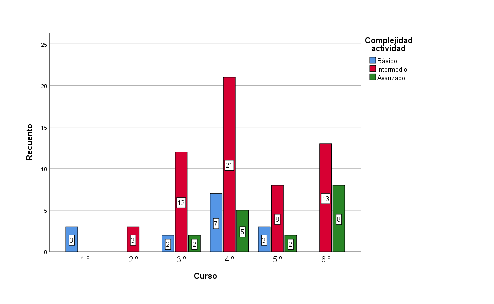
\includegraphics[width=0.85\textwidth]{Fig02.eps}
 \caption{Nivel de complejidad de las actividades por cursos.}
 \label{Fig02}
 \source{elaboración propia.}
\end{figure}

Por otro lado, en el \cref{Fig03} se advierte que las actividades digitales de los libros han puesto en marcha de forma mayoritaria la habilidad de comprensión escrita (CE) (95.5 \%), seguida por la de expresión escrita (EE) (77.5 \%); sin embargo la expresión oral (EO) (31.5 \%) y la comprensión oral (CO) (13.5 \%) se han fomentado en menor medida, en actividades como las siguientes: realización de exposiciones orales, elaboración de presentaciones informáticas en grupo o individual sobre un tema, consultas en diccionarios, enciclopedias digitales por parejas o en grupos, búsquedas de información en Internet sobre el ciberacoso o el uso de las tecnologías y la creación de tablas de datos o gráficos\footnote{Conviene aclarar que una misma actividad puede desarrollar más de una destreza, como se puede observar en la tabla 3; de ahí que los porcentajes del gráfico 3 sumen más del 100 \%.}. 

\begin{figure}[htbp]
 \centering
 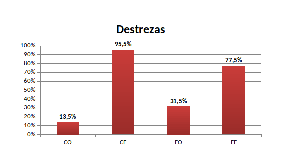
\includegraphics[width=0.65\textwidth]{Fig03.eps}
 \caption{Destrezas lingüísticas.}
 \label{Fig03}
 \source{elaboración propia.}
\end{figure}

Este resultado coincide, en parte, con lo referido en la Orden de 17 de marzo de 2015, en relación con el área de Lengua Castellana y Literatura, que insiste en la necesidad de que los aprendizajes tradicionales de lectura y escritura (bloques 2 y 3, respectivamente) se complementen con el uso de las TIC. Interesa, por tanto, saber qué destrezas lingüísticas se han utilizado en los distintos bloques temáticos establecidos para clasificar los contenidos digitales. 

La \cref{tbl03} muestra que, en general, todos los bloques temáticos de contenidos digitales se han trabajado de forma escrita, ya sea a través de la adquisición de la comprensión escrita (leer) como de la expresión escrita (escribir) o de ambas, ya que solo hay 1 actividad exclusivamente oral. De entre las que fomentan las destrezas escritas (de manera independiente o ambas), aparecen 44 actividades dedicadas a la búsqueda de información en Internet; 14 a trabajar el uso de las fuentes de información digitales (periódicos, revistas, enciclopedias digitales, diccionarios, etc.); 10 a tratar la utilización de la carta, el correo electrónico y el símbolo de arroba; 5 a la presentación oral de temas concretos; 6 al uso del procesador de textos para pasar actividades y realizar tablas o gráficos y 5, a la realización de exposiciones escritas sobre temas digitales. Finalmente, hay 4 actividades referidas a la denominación e imágenes de las tecnologías, de las cuales solo 1 es oral exclusivamente\footnote{En la tabla 3 aparece una actividad oral que, además, es la única de esta investigación. Pertenece a 2.º curso, 2.º trimestre y tiene como enunciado el siguiente: ¿Qué otras tecnologías, además del teléfono, permiten comunicarse? Dialoga sobre sus ventajas con tus compañeros. Le precede el símbolo del bocadillo, que indica interacción oral en el libro.}. Finalmente, la actividad dedicada a la interpretación de mensajes de teléfonos móviles trabaja destrezas escritas y orales. 

\begin{table}
\renewcommand{\arraystretch}{0.75}
\caption{Utilización de destrezas lingüísticas en los bloques temáticos de contenidos digitales.}
\label{tbl03}
\small
\begin{tabular}{p{0.2\textwidth}p{0.3\textwidth}cccc}
\toprule
 & & \multicolumn{3}{c}{Destrezas} & \multirow{2}{*}{Total} \\
 \cline{3-5}
 & & \begin{tabular}{@{}c@{}}Destrezas \\ escritas\end{tabular} & \begin{tabular}{@{}c@{}}Destrezas \\ orales\end{tabular} & Ambas \\
\midrule
\multirow{9}{*}{\begin{tabular}{@{}l@{}}Bloques temáticos de \\ los contenidos digitales\end{tabular}} & 1.Consultas o búsquedas de información en Internet & 30 & 0 & 14 & 44 \\
 & 2. Fuentes de información digitales & 11 & 0 & 3 & 14 \\
 & 3. Carta, correo electrónico y @ & 6 & 0 & 4 & 10 \\
 & 4. Presentación oral de temas & 2 & 0 & 3 & 5 \\
 & 5. Uso del procesador de textos. Gráficos y tablas. & 5 & 0 & 1 & 6 \\
 & 6. Exposiciones escritas sobre temas digitales & 4 & 0 & 1 & 5 \\
 & 7. Denominaciones o imágenes de las tecnologías & 2 & 1 & 1 & 4 \\
 & 8. Lectura e interpretación de mensajes de teléfonos móviles (WhatsApp) & 0 & 0 & 1 & 1 \\
\multicolumn{2}{c}{Total} & 60 & 1 & 28 & 89 \\
\bottomrule
\end{tabular}
\source{elaboración propia.}
\end{table}

Por otro lado, en el \cref{Fig04} se observa que la inmensa mayoría de las actividades de los libros son de carácter individual (78.7 \%); grupales solamente hay 9, que se corresponde con un 10.1 \% del total y en parejas un 4.5 \%. El último grupo está formado por 6 actividades, cinco de las cuales son tareas secuenciadas en las que primeramente se ha de realizar una tarea individual y seguidamente una grupal (recitación de un poema delante de los compañeros de clase, canto en el aula de un cuento de fórmula en forma de rap o de un poema en grupo, exposición oral de un tema al resto o realización de murales); y, finalmente una de ellas puede ser planteada por el docente en parejas o grupos, ya que no se especifica en el enunciado de la pregunta.

\begin{figure}[htb]
 \centering
 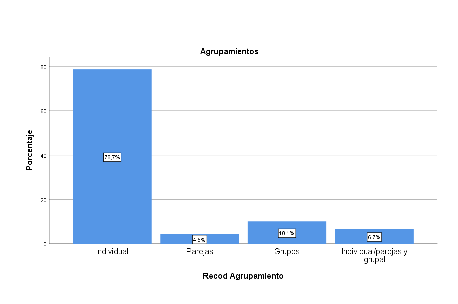
\includegraphics[width=0.75\textwidth]{Fig04.eps}
 \caption{Agrupamientos en las actividades.}
 \label{Fig04}
 \source{elaboración propia.}
\end{figure}

En cuanto a los bloques de contenido de los libros, ha llamado la atención que las actividades digitales se presenten, en su mayoría, en el bloque 1, dedicado a las Técnicas de estudio (33.7 \%), seguido por los bloques 3 (Repasa) y 4 (Literatura) (14.6 \%). Muy de cerca le sigue el bloque 6 de Expresión escrita (10.1 \%), el bloque 2 de Comprensión y expresión oral (Comunicación oral) (9 \%), los bloques especiales (8) (7.9 \%) y el bloque 5 sobre Conocimiento de la lengua (6.7 \%); obteniendo el peor resultado el bloque 7 de Lectoescritura (3.4 \%); como es lógico también, ya que solo había 3 actividades pertenecientes a este bloque. 

A la vista del \cref{Fig05}, resulta curioso que las actividades que trabajan las TIC en los libros se hayan incorporado mayoritariamente en el bloque de “Técnicas de estudio”, que aparece a partir de 3.º curso y cuya misión principal es la de ofrecer pautas para mejorar el estudio de los contenidos. 

\begin{figure}[htb]
 \centering
 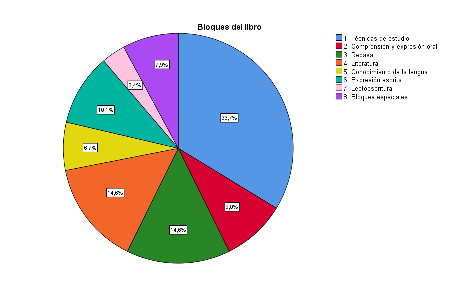
\includegraphics[width=0.65\textwidth]{Fig05.eps}
 \caption{Bloques del libro.}
 \label{Fig05}
 \source{elaboración propia.}
\end{figure}

Con el objeto de comprobar qué tipo de contenidos digitales son los que pertenecen a cada bloque del libro, se expone la \cref{tbl04}. En ella se observa que, efectivamente, el bloque de técnicas de estudio es el que prevalece sobre el resto con 30 actividades del total, 89; de las cuales, 22 pertenecen a actividades sobre búsquedas en Internet o el uso de fuentes de información digitales; 3 a la presentación oral de temas, 4 se reparten entre el estudio de la carta, el correo electrónico y el símbolo @ y el uso del procesador de textos y 1 sobre exposiciones escritas en Internet. Los bloques de Repasa y Literatura suman también una cifra importante (26 actividades), siendo 18 sobre la búsqueda de información en Internet. Sin embargo, es curioso que se dé tan poca importancia a los contenidos digitales en bloques tan representativos como el 2 (Comprensión y expresión oral), con solo 8 actividades (6 de ellas sobre búsquedas en Internet) o el 5 (Conocimiento de la lengua), con solo 6 actividades (3 de ellas también sobre búsquedas en Internet). Por su parte los bloques 6 (expresión escrita) y 7 (lectoescritura), solo suman 12 actividades del total, que se reparten mayoritariamente en el estudio de la carta, el correo electrónico y el símbolo @ (8 tareas), exposiciones escritas (2), el uso del procesador de textos (1) y las denominaciones digitales (1). Finalmente, en los bloques especiales de los libros (Conquista PISApolis, Emprende y Aprende, etc.) también aparecen actividades de contenido digital, siendo mayoritariamente búsquedas en Internet (5). 

\begin{table}[h!]
\renewcommand{\arraystretch}{0.9}
\caption{Tipo de contenidos digitales presentes en los bloques de los libros.}
\label{tbl04}
\small
\centering
\begin{tabular}{lllllllllll}
\toprule
 & & \multicolumn{8}{l}{Contenidos digitales} & Total \\
\cline{3-10}
 & & BI & FI & Cmail@ & PO & PTxt & ExEs & D/I Dig & SMS & \\
\midrule
\multirow{8}{*}{\begin{tabular}[l]{@{}l@{}}Bloques\\ del libro\end{tabular}} & 1.Técnicas de estudio &  12 & 10 & 2 & 3 & 2 & 1 & 0 & 0 & 30 \\
 & \begin{tabular}[l]{@{}l@{}}2.Comprensión y \\ expresión oral\end{tabular} &  6 & 0 & 0 & 0 & 0 & 0 & 2 & 0 & 8 \\
          & 3. Repasa                    & 7  & 1  & 0      & 2  & 2    & 1    & 0       & 0   & 13 \\
          & 4. Literatura                & 11 & 1  & 0      & 0  & 1    & 0    & 0       & 0   & 13 \\
          & \begin{tabular}[l]{@{}l@{}}5. Conocimiento \\ de la lengua\end{tabular} & 3  & 2  & 0      & 0  & 0    & 0    & 0       & 1   & 6  \\
          & 6. Expresión escrita         & 0  & 0  & 7      & 0  & 1    & 1    & 0       & 0   & 9  \\
          & 7. Lectoescritura            & 0  & 0  & 1      & 0  & 0    & 1    & 1       & 0   & 3  \\
          & 8.Bloques especiales         & 5  & 0  & 0      & 0  & 0    & 1    & 1       & 0   & 7  \\
\multicolumn{2}{l}{Total}                & 44 & 14 & 10     & 5  & 6    & 5    & 4       & 1   & 89 \\
\bottomrule
\end{tabular}
\source{elaboración propia.}
\end{table}

% Tabela desconfigurada na página
% Nota da tabela: BI= Búsquedas en Internet; FI= Fuentes de Información digitales; Cmail@= carta, correo electrónico y arroba; PO= Presentación oral de temas; PTxt= Uso del procesador de textos; ExEs= Exposiciones escritas sobre Internet; D/I Dig= Denominaciones o imágenes digitales; SMS = Mensajes de teléfonos móviles (WhatsApp)

En la \cref{tbl05} nos centramos en averiguar cómo son las actividades del bloque mayoritario, Técnicas de estudio, con el objeto de explicar mejor los resultados obtenidos.

\begin{small}
\renewcommand*{\arraystretch}{0.75}
\begin{longtable}{llllll}
\caption{Actividades del bloque Técnicas de estudio según contenidos digitales, curso y agrupamientos.}
\label{tbl05}
\\
\multicolumn{6}{l}{Bloque 1. Técnicas de estudio}\\
\toprule
 &  & \begin{tabular}[l]{@{}l@{}}Destrezas \\ escritas \end{tabular} & \begin{tabular}[l]{@{}l@{}}Destrezas \\ orales\end{tabular} & Ambas & Total \\
\midrule
Contenidos digitales & Búsquedas en Internet                                                           & 11                 &                  & 1     & 12    \\
                     & \begin{tabular}[c]{@{}l@{}}Fuentes de información \\ digitales\end{tabular}     & 9                  &                  & 1     & 10    \\
                     & \begin{tabular}[c]{@{}l@{}}Carta, correo electrónico y \\ @\end{tabular}        & 1                  &                  & 1     & 2     \\
                     & Presentación oral de temas                                                      & 2                  &                  & 1     & 3     \\
                     & \begin{tabular}[c]{@{}l@{}}Uso del procesador de \\ textos\end{tabular}         & 2                  &                  & 0     & 1     \\
                     & \begin{tabular}[c]{@{}l@{}}Exposiciones escritas \\ sobre Internet\end{tabular} & 1                  &                  & 0     & 1     \\
                     & Total                                                                           & 26                 &                  & 4     & 30    \\
\midrule
Curso                & 3.º                                                                             & 7                  &                  & 1     & 8     \\
                     & 4.º                                                                             & 13                 &                  & 1     & 14    \\
                     & 5.º                                                                             & 2                  &                  & 0     & 2     \\
                     & 6.º                                                                             & 4                  &                  & 2     & 6     \\
                     & Total                                                                           & 26                 &                  & 4     & 30    \\
\midrule
Agrupamientos & Individual                 & 25 &  & 3 & 28 \\
              & Parejas                    & 0  &  & 1 & 1  \\
              & Grupos                     & 1  &  & 0 & 1  \\
              & Total                      & 26 &  & 4 & 30 \\
\bottomrule
\source{elaboración propia.}
\end{longtable}
\end{small}

% Tabela desconfigurada

Los resultados revelan que en este bloque todas las actividades, con independencia del contenido digital, desarrollan solamente destrezas escritas, ya sea comprensión/ expresión escrita o ambas. Además, pertenecen en su mayoría a 3.º o 4.º curso y son de carácter individual, ya que solo existe una grupal. Esto hace pensar que, dado que la etapa educativa estudiada es Educación Primaria, la introducción de contenidos digitales haya preferido realizarse de forma sutil en este bloque, a través de búsquedas en Internet o el uso de fuentes de información diversas a través de la red, como tareas de estudio de los contenidos aprendidos en la unidad; y con la finalidad de iniciar a los estudiantes de 3.º curso en adelante en el uso de las tecnologías, que desarrollarán más tarde en Educación Secundaria. Sin obviar, claro está, las actividades de los bloques de Literatura y Repasa, que también suman una cifra destacada. Parece, por tanto, que las tecnologías en Educación Primaria se están estudiando en la editorial Edelvives de forma transversal para aprender contenidos literarios, aplicar técnicas de estudio o repasar aprendizajes.

\section{Discusión y conclusiones}\label{sec-conclusao}
En este estudio se ha analizado la presencia de las tecnologías en los libros de texto de Lengua Castellana y Literatura del proyecto educativo Superpixépolis de la editorial Edelvives. Concretamente, se han considerado los 16 manuales de Lengua Castellana y Literatura de Educación Primaria que contenían actividades tecnológicas de distintos trimestres. Se pretendía conocer, fundamentalmente, los contenidos digitales que trabajaban en función de diferentes variables de análisis: el curso, el bloque del libro, el tipo de complejidad de la actividad, las destrezas y el agrupamiento. 

\textcite{marin_diaz_universidad_2012} afirman que las TIC son beneficiosas para el proceso de enseñanza-aprendizaje, ya que constituyen una herramienta útil para aprender, elaborar trabajos, actividades, ejercicios, etc. Sin duda, dicha utilidad se ha demostrado en esta investigación, ya que ha habido una presencia importante de actividades digitales en los manuales (N= 89), pese a centrarse en la etapa de Educación Primaria, que cuenta con un alumnado de entre 6-12 años. Obviamente, está demostrado que el uso de las tecnologías de la información y la comunicación en la práctica de aula aumenta la atención, la motivación y la participación del alumnado \cite{domingo-coscollola_classroom_2011}, facilita la creación de conocimiento colectivo \cite{gairin_sallan_2010} y mejora sus aprendizajes y rendimiento académico \cite{prats_i_fernandez_pueden_2015}. Lógicamente, el uso de Internet para consultas diversas o de los procesadores de textos (Word o PowerPoint) motivan al estudiante, puesto que el aprendizaje convencional de contenidos de un libro de texto se engrandece con una fuente inagotable de conocimiento en la red que, por supuesto, han de conocer y valorar convenientemente. Luque de \textcite{luque_de_la_rosa_tecnologias_2015} reconocen el carácter educativo del uso de internet en alumnado de primaria y su valor positivo para el rendimiento académico. 
A la vista de los resultados obtenidos en esta investigación, podemos señalar que los bloques temáticos en los que se han agrupado los contenidos digitales de los libros han sido los siguientes: 

\begin{enumerate}
    \item Consultas o búsquedas de información en Internet para extraer datos, interpretar información, relacionar investigaciones concretas, hacer lecturas de formularios, blogs, páginas web; realización de traducciones o audiciones de poemas.
    \item Fuentes de información digitales: periódicos, revistas, enciclopedias digitales, diccionarios, buscadores, etc.
    \item La carta, el correo electrónico y el símbolo de arroba: definición, estructura y diferenciación.
    \item Presentación informática/digital (oral) de un tema a través de Microsoft Powerpoint sobre temas diversos.
    \item Uso del procesador de textos. Tablas y gráficos: escritura de cuentos literarios o realización de anuncios sobre productos a ordenador. Creación de tablas y gráficos en Microsoft Word. 
    \item Exposiciones escritas sobre Internet acerca de la utilidad de Internet, la búsqueda de información en la red, la utilidad de móviles, tabletas y ordenadores, los ciberdelitos y ciberacosos o el uso desaconsejable del móvil en determinados contextos.
    \item Denominaciones e imágenes de las tecnologías: términos digitales o imágenes sobre tecnologías, por ejemplo «teléfono» o «teclado».
    \item Lectura e interpretación de mensajes de teléfonos móviles: uso de WhatsApp (no explícito).
\end{enumerate}

\textcite{marques_graells_nueva_2007} ya señalaba una serie de conocimientos y competencias básicas en TIC, entre las que se encontraban algunos de los contenidos de los libros estudiados: uso del procesador de textos, navegación en Internet (búsqueda y selección de información), uso del correo electrónico, elaboración de documentos multimedia (presentaciones) y conocimiento básico de la hoja de cálculo y bases de datos. En otros estudios también se aluden a contenidos idénticos o similares a los mencionados. \textcite{fernandez-montalvo_habitos_2015} manifiestan encontrar conductas de acoso importantes en alumnos de 6.º de Primaria, puesto que el 9.4 \% dice haber recibido amenazas por correo electrónico, el 13.7 \% haber sido insultado a través de la Red e incluso un 12.3 \% reconoce haber insultado ellos mismos a otros compañeros a través de Internet. De ahí la necesidad de poner en marcha un programa de alfabetización digital como el propuesto por \textcite{fernandez-montalvo_effectiveness_2017}. Tras él, se observa que los participantes muestran un mayor grado de conocimiento sobre los peligros derivados del uso de Internet, unas medidas de privacidad adecuadas y unos comportamientos relacionados con el acoso. Además, \textcite{gamiz_sanchez_estudio_2016} en su investigación concluyen que un 47 \% de los alumnos del primer ciclo encuestados son capaces de realizar escritos haciendo uso del procesador de texto. Igualmente es de destacar que el 43 \% de ellos utilizan el ordenador para realizar actividades de aprendizaje como leer o escribir; sin embargo, el 86 \% no sabe hacer una presentación multimedia y solo un 10 \% hace uso del correo electrónico. Igualmente, el 52 \% ha utilizado alguna enciclopedia o diccionario en la red. 

Los resultados de esta investigación revelan la aparición de actividades grupales en tercer curso que se centran en la investigación y presentación informática posterior de cualquiera de estos dos temas propuestos: el ciclo del agua o la elaboración del pan. Al respecto, \textcite{martin_garcia_alisis_2016} habla de la utilización de vídeos por parte del docente para la generación posterior de debates y reflexiones grupales y de actividades por grupos centradas en la elaboración de presentaciones multimedia a través de Microsoft PowerPoint. Igualmente, la presentación Powerpoint también es un recurso utilizado por docentes para presentar sus lecciones, al igual que páginas web y recursos en Internet \cite{trujillo_torres_caracterizacion_2011}.

Además, se ha verificado que la presencia mayoritaria de estos bloques temáticos de contenidos digitales se encontraba a partir del último curso del segundo ciclo y en el tercer ciclo de Primaria, ya que ha sido en 4.º (37.1 \%), 5.º (14.6 \%) y 6.º curso (23.6 \%) donde se han obtenido cifras mayores; frente al primer ciclo de Primaria, donde los contenidos digitales han sido mínimos (6.8 \%). Es lógico de suponer también, ya que a medida que los niños poseen más edad existen más posibilidades de entender contenidos más complejos como son, en este caso, los tecnológicos. 

Además, los resultados han arrojado información acerca de la complejidad de las actividades por cursos, y si bien es cierto que ha predominado el nivel intermedio, según el DigComp 2.1 \cite{carretero_2018}, ha sido en 3.º (12), 4.º (21) y 6.º (13) donde más actividades de este grado de complejidad se han dado; destacándose un incremento de tareas de nivel avanzado en 6.º curso (8 actividades/13 de nivel intermedio), frente a la nula presencia de ellas en el primer ciclo. 

Los datos también han mostrado que las destrezas que ha puesto en marcha el alumnado a la hora de realizar las actividades han sido fundamentalmente las escritas: comprensión escrita (95.5 \%) y expresión escrita (77.5 \%), potenciándose así tareas desde unir con flechas o colorear letras a escribir exposiciones sobre un tema, responder por escrito a preguntas, escribir fichas, anotar datos, redactar cuentos, escribir tecleando en el ordenador para buscar información en la red o para hacer una presentación Powerpoint. De entre estas actividades han prevalecido mayormente las dedicadas a la búsqueda de información en Internet o al uso de fuentes de información digitales. \textcite{calcines_pinero_integracion_2016} llegan a conclusiones similares cuando afirman que la tipología de actividades más motivadoras para el alumnado de su estudio han sido aquellas que trabajaban con medios audiovisuales y tecnológicos (búsquedas por Internet, uso del móvil, pizarra digital o vídeos). 

En cuanto a los agrupamientos, no se ha potenciado el trabajo en grupos (10.1 \%) o por parejas (4.5 \%) prácticamente nada, ya que un 78.7 \% de las actividades son individuales. Únicamente hay 6 actividades que alternan el trabajo individual y por parejas o grupal (búsqueda de información grupal sobre el uso de móviles, tabletas u ordenadores o sobre temas como el ciberacoso o lectura e interpretación de mensajes de teléfonos móviles mediante interacción oral con compañeros). La carencia de este tipo de actividades nos permite concluir que el proyecto educativo Superpixépolis de Edelvives no fomenta la participación en clase ni la cooperación entre compañeros y profesores, evitando así la creación de un ecosistema colaborativo \cite{marin_diaz_universidad_2012}. \textcite{diaz_lazaro_social_2016} advierte que el alumnado prefiere trabajar en grupo, ya que desarrolla sus habilidades sociales y de comunicación y promueve la construcción compartida del conocimiento.  

Por otro lado, y una vez recodificados los bloques de contenido de los libros que aparecían en el índice, se han obtenido los siguientes: 1. Técnicas de estudio (33.7 \%); 2. Comprensión y expresión oral (9 \%); 3. Repasa (14.6 \%); 4. Literatura (14.6 \%); 5. Conocimiento de la lengua (6.7 \%); 6. Expresión escrita (10.1 \%); 7. Lectoescritura (3.4 \%) y 8. Bloques especiales (7.9 \%). Los datos arrojan información llamativa, puesto que la mayoría de las actividades digitales se incorporan en el bloque de Técnicas de estudio, y entre ellas destacan las de búsqueda en Internet y las de fuentes de información digitales. Igualmente los bloques de Repasa y Literatura también son excusa para plantear tareas tecnológicas; en el resto de bloques la presencia es menor. Se trata de actividades sobre técnicas de estudio que pertenecen a 3.º o 4.º curso, son escritas y de carácter individual. 

Finalmente, en cuanto a las limitaciones del estudio se encuentra principalmente el haber analizado exclusivamente el proyecto educativo de una editorial, Edelvives, para la asignatura de Lengua Castellana y Literatura en Educación Primaria. Por tanto, para futuras investigaciones sería fundamental comparar este proyecto educativo con otros más recientes de la misma editorial y con los proyectos educativos de Lengua Castellana y Literatura para Primaria de otras editoriales, con el objeto de observar qué novedades tecnológicas se introducen así como el enfoque utilizado. Asimismo, resulta interesante contrastar estos resultados con los de otras provincias andaluzas, en particular, y españolas, en general, que también hayan estudiado la presencia de contenidos digitales en libros de texto de Primaria de cualquier área de conocimiento. Finalmente, sería relevante realizar más investigaciones de carácter mixto (cualitativo/cuantitativo), que ofrezcan información acerca del tipo de actividades digitales de los libros de texto antes de que se dé el paso definitivo en la industria editorial al formato digital.

\section{Agradecimientos}\label{sec-agradecimento}
Esta investigación está respaldada por el Grupo de Investigación HUM-457 (Didáctica de la Lengua y la Literatura) de la Facultad de Ciencias de la Educación de la Universidad de Granada (España).

\printbibliography\label{sec-bib}

\end{document}
